\documentclass[10pt,a4paper]{article}
\usepackage[utf8]{inputenc}
\usepackage[italian]{babel}
\usepackage{amsmath}
\usepackage{amsfonts}

\usepackage{siunitx}
\usepackage{amssymb}
\usepackage{graphicx}


\DeclareGraphicsExtensions{.pdf}

\begin{document}

\author{Riccardo Antonelli, Federico Chiossi, Patato Schiavi}
\title{Timing}

\maketitle

\section{Obiettivi}

% misura andamento del guadagno dei PMT in funzione della tensione applicata determinando il punto di lavoro ottimale
% determinare la calibrazione in energia degli scint organici e la ris energetica dell'analisi dei Compton edge
% determinare ritardo esterno CFTD che ottimizza la ris t del sistema
% determinare andamento ris temporale in f del range dinamico dei segnali analizzati dal CFTD

\begin{itemize}

\item Misura dell'andamento del guadagno dei PMT in funzione della tensione applicata e determinazione del punto di lavoro ottimale
\item determinazione della calibrazione in energia degli scintillatori organici e la risoluzione energetica dell'analisi dei Compton edge
\item determinazione del ritardo esterno CFTD che ottimizza la risoluzione temporale del sistema
\item determinazione dell'andamento della risoluzione temporale in funzione del range dinamico dei segnali analizzati dal CFTD

\end{itemize}

\section{Fit del profilo Compton}

In aggiunta al metodo consigliato per la stima della risoluzione energetica e della posizione del picco Compton per la calibrazione (metodo \textbf{SEMIGAUSS}) basato sul fit di una mezza Gaussiana e relativa correzione dell'imprecisione, abbiamo sviluppato un metodo alternativo (metodo \textbf{FIT}) basato su un fit esplicito di un profilo Compton.\\

Come profilo energetico "grezzo" (senza considerare la risoluzione dell'apparato) abbiamo considerato la seguente distribuzione. Definiamo $\text{edge}_{1,2} \approx \SI{340}{\kilo\electronvolt}, \SI{1062}{\kilo\electronvolt}$ gli edge Compton per i fotoni rispettivamente a $511$ e $\SI{1275}{\kilo\electronvolt}$. Se $c$ è il canale, e $(y,e_1,e_2,k)$ sono parametri che descrivono la distribuzione, definiamo

\[E_0 := \left(\text{edge}_1 - \frac{e_1}{e_2} \, \text{edge}_2\right)/\left(1-\frac{e_1}{e_2}\right) \]

$E_0$ è semplicemente la stima dell'energia al canale $0$. I parametri $e_i$ sono le posizioni in canali dei due Compton edge.

\[E(c) := E_0 + \left(\frac{\text{edge}_1 - E}{e_1}\right) c\]

$E(c)$ è la stima dell'energia al canale $c$. Notare che abbiamo semplicemente effettuato la calibrazione tale per cui $E(e_i) = \text{edge}_i$.\\

A questo punto definiamo la distribuzione

\[ A(c) := y \sum_i k_i \left( 2-2 \frac {E} {\epsilon_i - E} + \frac{E^2}{(\epsilon_i-E)^2} + \frac{E^2}{\epsilon_i (\epsilon_i-E)} \right) \chi(c<e_i) \]

La somma è sui due picchi Compton; $k_1 = 1$ e $k_2 = k$, parametro che racchiude il rapporto in ampiezza fra i due picchi Compton. $y$ è un fattore di scala globale sulle frequenze. $\epsilon_i$ sono le energie dei fotoni, $\sim 1275$ e $\SI{511}{\kilo\electronvolt}$. $\chi$ è una funzione indicatrice che tronca il profilo in corrispondenza del picco Compton.\\

Per tenere conto della risoluzione dello strumento abbiamo inizialmente effettuato una convoluzione del profilo $A(c)$ con una gaussiana di integrale unitario. Questa nuova distribuzione ha un parametro addizionale, la deviazione standard della gaussiana $\sigma$:

\[ B(c;y,e_1,e_2,k,\sigma) = A(c;y,e_1,e_2,k) * \text{gauss}(c';\sigma) \]

Questo modello non fittava bene i dati. Alla luce del fatto che la risoluzione energetica è essa stessa dipendente dall'energia, abbiamo immaginato che la $\sigma$ fosse una funzione lineare del canale:

\[ \sigma(c) = \gamma c \]

Con $\gamma$ un parametro adimensionale. Per cui la distribuzione risultante è

\[ B(c; y, e_1, e_2, k ,\gamma) = A(c;y,e_1,e_2,k) * \text{gauss}(c';\gamma c) \]

(la scrittura è formale, dal momento che non si tratta più di una convoluzione vera e propria.) Nel dettaglio il calcolo effettuato è stato

\[ B(c) = \sum_j A(c+j)\,  \text{gauss}(j;\gamma c) \]

con un range ragionevole per $j$.\\

La distribuzione finale è stata fittata ai dati mediante un metodo a forza bruta; lo spazio dei parametri è stato diviso in celle e le celle sono state esplorate per trovare il set che minimizzava lo scarto quadratico totale. Successivamente si ripeteva la ricerca raffinando la griglia.

\section{Analisi}

\subsection{Guadagno - Voltaggio}



\subsection{Calibrazione energetica}

In grafico riportiamo il parametro $\sigma / \text{canali}$ stimato con il metodo ??? in funzione del voltaggio.


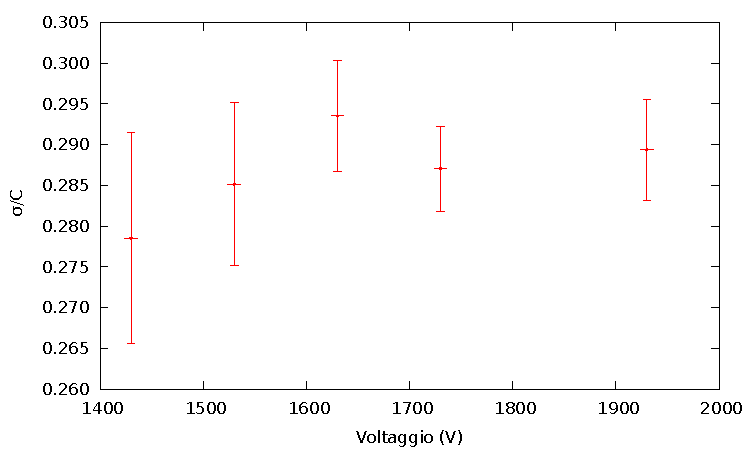
\includegraphics[scale=1]{../out/chio/Guadagno_R1}

Notiamo che non è possibile dedurre la presenza di un minimo.

\subsection{Risoluzione temporale}

Vogliamo determinare il ritardo che ottimizza la risoluzione temporale dell'apparato.\\

La calibrazione temporale è stata effettuata acquisendo lo spettro temporale del TAC variando il delay utilizzando ritardi predefiniti. Dopodiché fittiamo una gaussiana su ogni spettro; infine fittiamo il ritardo noto con i centroidi ottenuti:

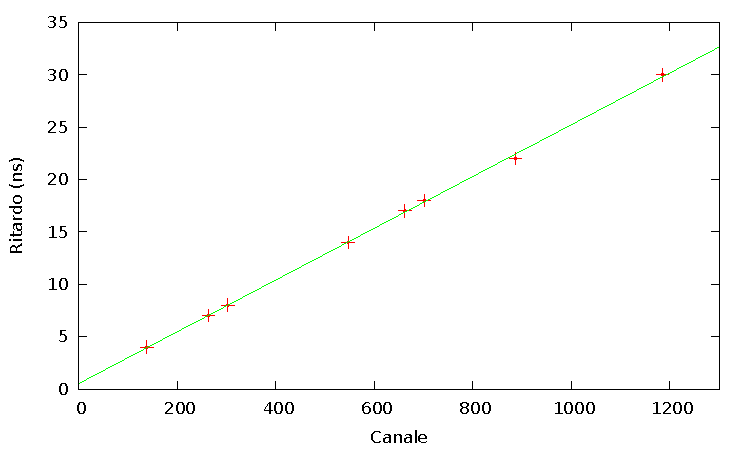
\includegraphics[scale=1]{../out/chio/Cal_DnDt}

Risulta $t = (0.0247 \pm 0.0002)\, \si{\nano\second}\,\mathrm{canali}^{-1} \cdot C + (0.53 \pm 0.16 \, \si{\nano\second})$.\\

\`E necessario stimare inoltre il ritardo corrispondente ai cavi LEMO. Fittiamo il ritardo misurato con la lunghezza totale di LEMO:

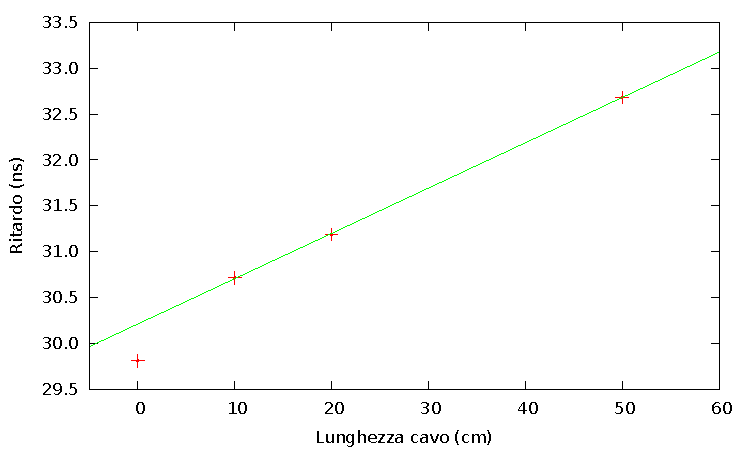
\includegraphics[scale=1]{../out/chio/tempo_residui}


\section{Conclusioni}

\end{document}